%%%%%%%%%%%%%%%%%%%%%%%%%%%%%%%%%%%%%%%%%%%%%%%%%%%%%%%%%%%%%%%%%%%%%
%% This is a (brief) model paper using the achemso class
%% The document class accepts keyval options, which should include
%% the target journal and optionally the manuscript type. 
%%%%%%%%%%%%%%%%%%%%%%%%%%%%%%%%%%%%%%%%%%%%%%%%%%%%%%%%%%%%%%%%%%%%%

% Use single column for preprint.
\documentclass[journal=jpca,manuscript=article,layout=singlecolumn]{achemso}

%%%%%%%%%%%%%%%%%%%%%%%%%%%%%%%%%%%%%%%%%%%%%%%%%%%%%%%%%%%%%%%%%%%%%
%% Place any additional packages needed here.  Only include packages
%% which are essential, to avoid problems later. Do NOT use any
%% packages which require e-TeX (for example etoolbox): the e-TeX
%% extensions are not currently available on the ACS conversion
%% servers.
%%%%%%%%%%%%%%%%%%%%%%%%%%%%%%%%%%%%%%%%%%%%%%%%%%%%%%%%%%%%%%%%%%%%%
\usepackage{amsmath}
\usepackage{amssymb}
\usepackage{bbm}
\usepackage{booktabs}
\usepackage{placeins}
\usepackage{siunitx}
\usepackage{xcolor}
\usepackage{xr}

%%%%%%%%%%%%%%%%%%%%%%%%%%%%%%%%%%%%%%%%%%%%%%%%%%%%%%%%%%%%%%%%%%%%%
%% If issues arise when submitting your manuscript, you may want to
%% un-comment the next line.  This provides information on the
%% version of every file you have used.
%%%%%%%%%%%%%%%%%%%%%%%%%%%%%%%%%%%%%%%%%%%%%%%%%%%%%%%%%%%%%%%%%%%%%
%%\listfiles

%%%%%%%%%%%%%%%%%%%%%%%%%%%%%%%%%%%%%%%%%%%%%%%%%%%%%%%%%%%%%%%%%%%%%
%% Place any additional macros here.  Please use \newcommand* where
%% possible, and avoid layout-changing macros (which are not used
%% when typesetting).
%%%%%%%%%%%%%%%%%%%%%%%%%%%%%%%%%%%%%%%%%%%%%%%%%%%%%%%%%%%%%%%%%%%%%
\newcommand*\mycommand[1]{\texttt{\emph{#1}}}
\DeclareMathOperator{\Var}{Var}
\DeclareMathOperator{\tr}{tr}
\DeclareMathOperator{\Span}{span}
\DeclareMathOperator{\Div}{div}
\DeclareMathOperator{\Diag}{diag}
\DeclareMathOperator{\Id}{\mathbf{1}}
\DeclareMathOperator*{\argmin}{arg\,min}

% bold matrix
\newcommand\m[1]{\mathbf{#1}}
% bold vector
\renewcommand\vec[1]{\mathbf{#1}}

\setkeys{acs}{doi = true}
\SectionNumbersOn

% Equations in the SI should be labeled as SI-1, SI-2
% to distinguish them from the equations in the main text.
\renewcommand{\theequation}{SI-\arabic{equation}}
% Figures and tables in the SI should be labeled as S1, S2.
\renewcommand{\thefigure}{S\arabic{figure}}
\renewcommand{\thetable}{S\arabic{table}}

% For referring to equations in the main text
\makeatletter
\newcommand*{\addFileDependency}[1]{% argument=file name and extension
  \typeout{(#1)}
  \@addtofilelist{#1}
  \IfFileExists{#1}{}{\typeout{No file #1.}}
}
\makeatother

\newcommand*{\myexternaldocument}[1]{%
    \externaldocument{#1}%
    \addFileDependency{#1.tex}%
    \addFileDependency{#1.aux}%
}
\myexternaldocument{main_long_version}

%%%%%%%%%%%%%%%%%%%%%%%%%%%%%%%%%%%%%%%%%%%%%%%%%%%%%%%%%%%%%%%%%%%%%
%% Meta-data block
%% ---------------
%% Each author should be given as a separate \author command.
%%
%% Corresponding authors should have an e-mail given after the author
%% name as an \email command. Phone and fax numbers can be given
%% using \phone and \fax, respectively; this information is optional.
%%
%% The affiliation of authors is given after the authors; each
%% \affiliation command applies to all preceding authors not already
%% assigned an affiliation.
%%
%% The affiliation takes an option argument for the short name.  This
%% will typically be something like "University of Somewhere".
%%
%% The \altaffiliation macro should be used for new address, etc.
%% On the other hand, \alsoaffiliation is used on a per author basis
%% when authors are associated with multiple institutions.
%%%%%%%%%%%%%%%%%%%%%%%%%%%%%%%%%%%%%%%%%%%%%%%%%%%%%%%%%%%%%%%%%%%%%
\author{Alexander Humeniuk}
\email{alexander.humeniuk@gmail.com}
\affiliation[]
{Department of Chemistry, Graduate School of Science, Kyoto University, Kitashirakawa-Oiwakecho, Sakyo-Ku, Kyoto 606-8502, Japan}

%%%%%%%%%%%%%%%%%%%%%%%%%%%%%%%%%%%%%%%%%%%%%%%%%%%%%%%%%%%%%%%%%%%%%
%% The document title should be given as usual. Some journals require
%% a running title from the author: this should be supplied as an
%% optional argument to \title.
%%%%%%%%%%%%%%%%%%%%%%%%%%%%%%%%%%%%%%%%%%%%%%%%%%%%%%%%%%%%%%%%%%%%%
\title[]
  {Supporting Information for 'Approximate functionals for multistate density functional theory'}

%%%%%%%%%%%%%%%%%%%%%%%%%%%%%%%%%%%%%%%%%%%%%%%%%%%%%%%%%%%%%%%%%%%%%
%% Some journals require a list of abbreviations or keywords to be
%% supplied. These should be set up here, and will be printed after
%% the title and author information, if needed.
%%%%%%%%%%%%%%%%%%%%%%%%%%%%%%%%%%%%%%%%%%%%%%%%%%%%%%%%%%%%%%%%%%%%%
\abbreviations{}
\keywords{}

%%%%%%%%%%%%%%%%%%%%%%%%%%%%%%%%%%%%%%%%%%%%%%%%%%%%%%%%%%%%%%%%%%%%%
%% The manuscript does not need to include \maketitle, which is
%% executed automatically.
%%%%%%%%%%%%%%%%%%%%%%%%%%%%%%%%%%%%%%%%%%%%%%%%%%%%%%%%%%%%%%%%%%%%%
\begin{document}

\section{Electron Repulsion}

\subsection{Correlation Functional}
\begin{figure}[h!]
  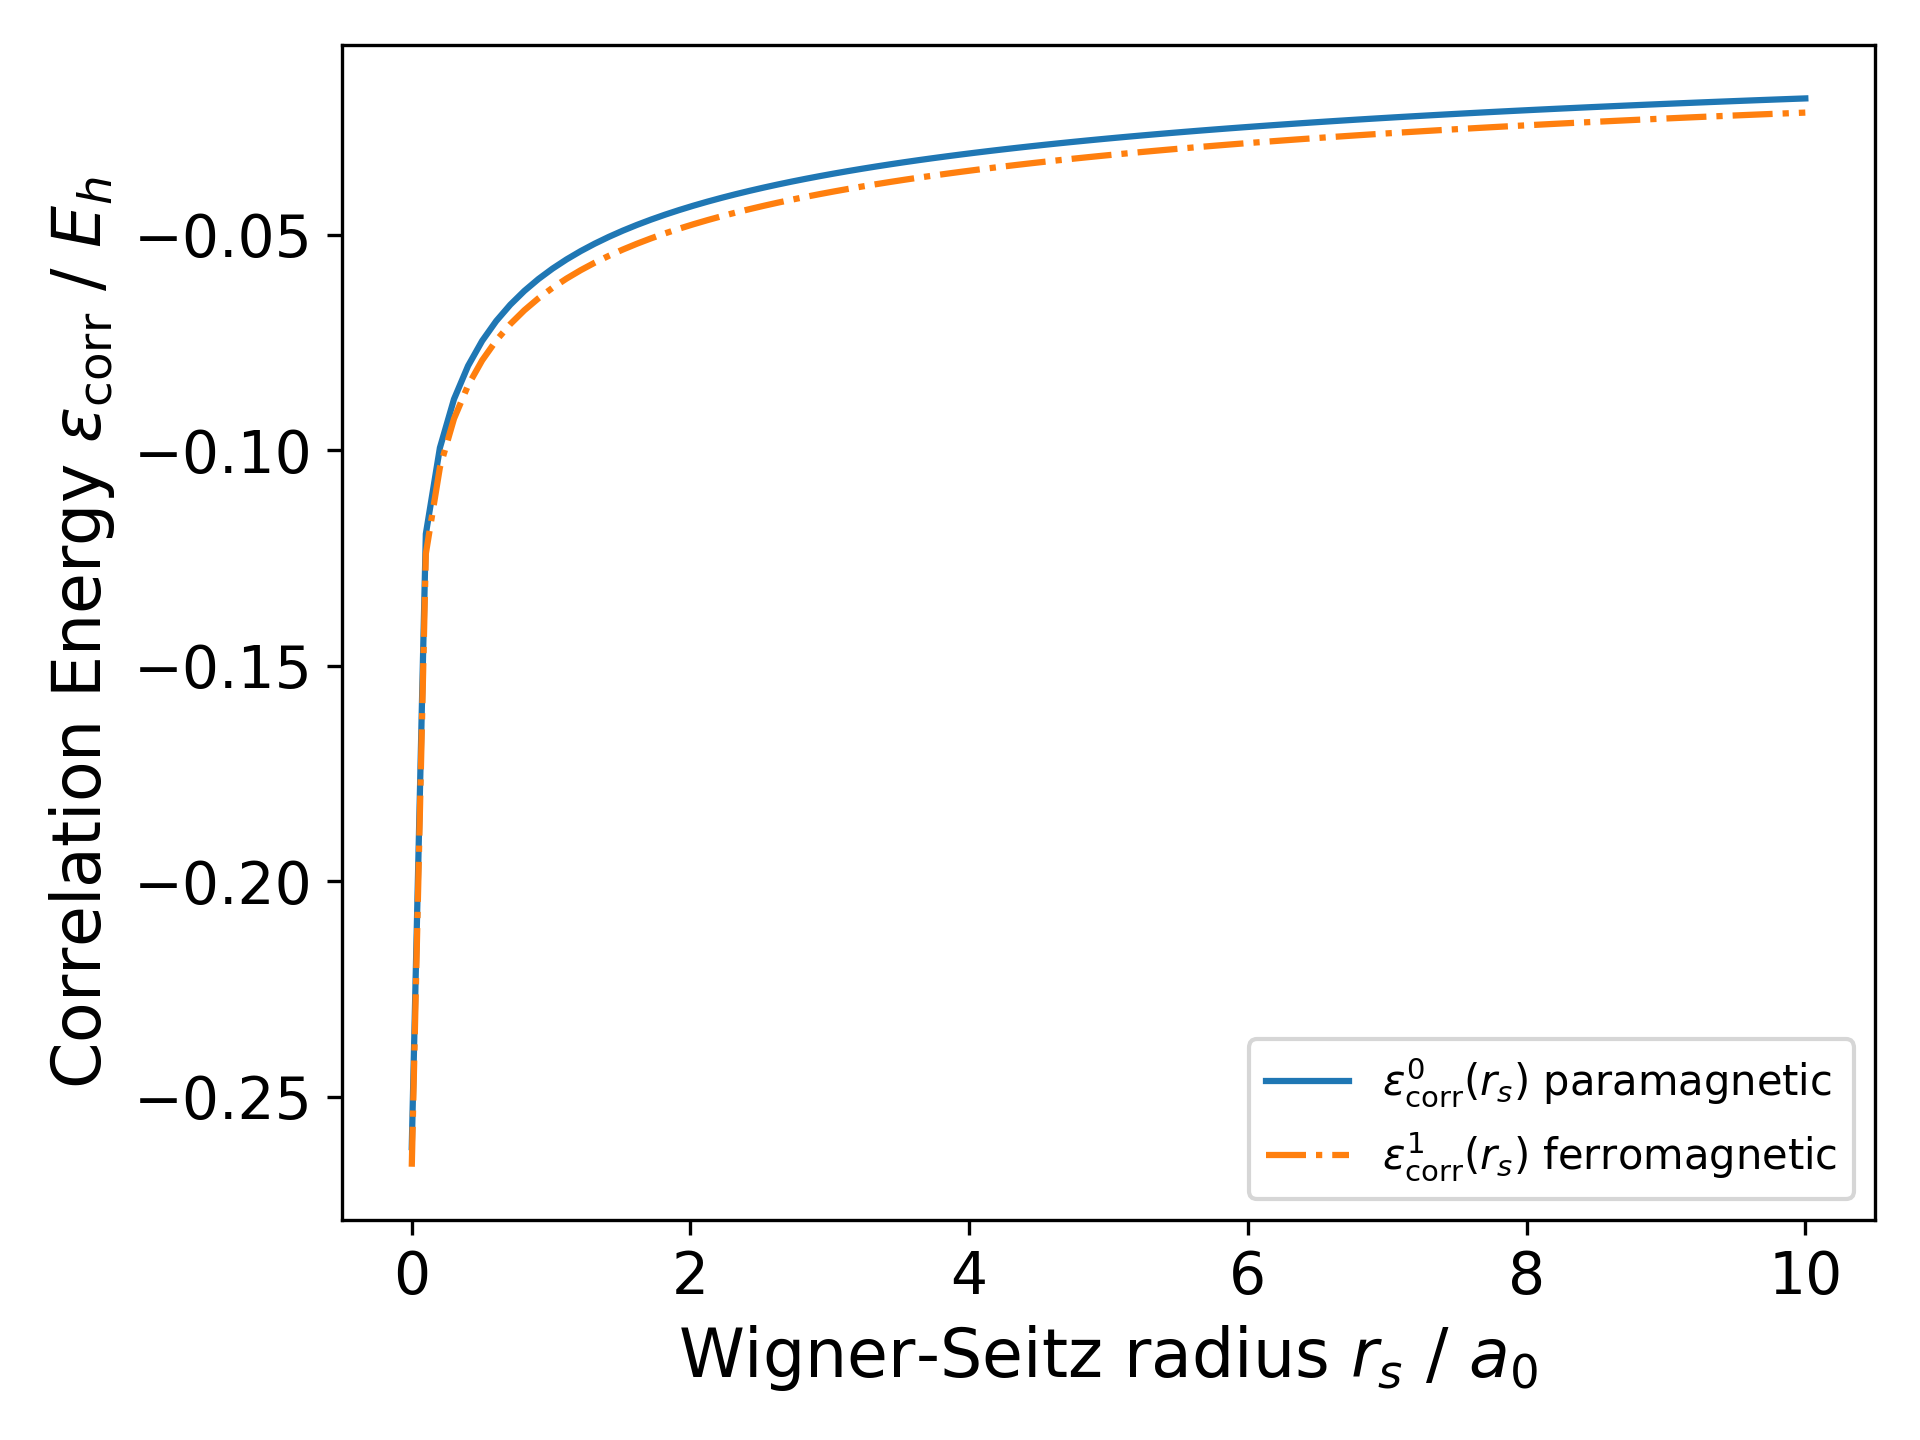
\includegraphics[width=0.5\linewidth]{figures/correlation_energy_paramagnetic_fs_ferromagnetic.png}
  \caption{\label{fig:correlation_energy_paramagnetic_fs_ferromagnetic}
  Paramagnetic (spin polarization $\zeta=0$) and ferromagnetic $\zeta=1$) correlation energy per particle
  $\epsilon_{\text{corr}}^{\zeta}$
  of a uniform electron gas with density $\rho = \frac{3}{4 \pi} r_s^{-3}$.
  The parameterization of Chachiyo \cite{Chachiyo2016} is used.}
\end{figure}
\FloatBarrier

\subsection{Klein's trace inequality}
\label{sec:Kleins_inequality}
Klein's inequality \cite{wiki:Kleins_inequality} \cite{Ruelle1969statistical} states that given two Hermitian, positive-definite $N \times N$ matrices $\m{A}$ and $\m{B}$ and
a convex function $f: \mathbb{R} \mapsto \mathbb{R}$ with derivative $f'$ the following trace inequality holds,
\begin{equation}
\tr\left[ f(\m{A}) - f(\m{B}) - (\m{A} - \m{B}) f'(\m{B}) \right] \ge 0 \label{eqn:Kleins_inequality}.
\end{equation}
With $f(x) = x^{4/3}$ (so that $f'(x) = 4/3 x^{1/3}$) and $\m{A} = \m{D}$ (full matrix) and $\m{B} = \Diag(\m{D}) = \Diag(D_{00}, D_{11}, \ldots, D_{NN})$ (only diagonal elements),
Klein's inequality becomes
\begin{equation}
\tr\left[ \m{D}^{4/3} - \Diag(\m{D})^{4/3} \right] \ge \tr\left[ \frac{4}{3} \left(\m{D} - \Diag(\m{D})\right) \Diag(\m{D})^{1/3}\right].
\end{equation}
The right hand side of this inequality is zero, since $\tr(\m{D} \Diag(\m{D})^{1/3}) = \tr(\Diag(\m{D})^{4/3})$, so that 
\begin{equation}
\tr(\m{D}^{4/3}(\vec{r})) \ge \sum_I D_{II}(\vec{r})^{4/3}.
\end{equation}
Integrating over space yields the inequality \ref{eqn:K_inequality}.

\subsection{Lower Bound of Electron Repulsion Energy}
\label{sec:lieb_oxford_bound_electron_repulsion}
%%%%% This digression can be moved to the SI.
The proof that the Lieb-Oxford bound also works for density matrices is not spelled out explicitly in Ref.~\cite{Lieb1981}. To be sure, a proof
of inequality \ref{eqn:lieb_oxford_bound_subspace_invariant} will be sketched that uses the ideas of Lieb and Oxford. The original publications
\cite{Lieb1979,Lieb1981} are written in a very dense style. A more accessible explanation of the proof
for a less tight bound is given in chapter 6 of E. Lieb's book "Stability of Matter in Quantum Mechanics" \cite{Lieb2010_Stability_of_Matter}.
I will follow the notation of the book, except for denoting the Coulomb interaction between two charge densities
$f(\vec{r})$ and $g(\vec{r})$ by 
\begin{equation}
  C(f,g) = \frac{1}{2} \int d^3r \int d^3r' \frac{f(\vec{r}) g(\vec{r}')}{\vert \vec{r} - \vec{r}' \vert}
\end{equation}
(instead of $D(f,g)$) to avoid confusion with the matrix density. The starting point is Onsager's lemma
(Lemma 6.1 in \cite{Lieb2010_Stability_of_Matter}), which is valid for any charge density. For our purposes the
charge density is set to the subspace density $\rho_V$,
\begin{equation}
\frac{1}{2} \sum_{i \neq j}^n \frac{1}{\vert \vec{r}_i - \vec{r}_j \vert}
\geq - C(\rho_V,\rho_V) + 2 \sum_{i=1}^n C(\rho_V, \mu_{\vec{r}_i}) - \sum_{i=1}^{n} C(\mu_{\vec{r}_i},\mu_{\vec{r}_i}) \label{eqn:onsagers_lemma}
\end{equation}
The $\mu_{\vec{r}_i}(\vec{r})$ are bounded and normalized ($\int d^3r \mu_{\vec{r}_i}(\vec{r}) = 1$) functions, which are
spherically symmetric around the position $\vec{r}_i$ of electron $i=1,\ldots,n$.
They can be understood as the smeared out charge of an electron. The inequality is useful, because
the 2-electron repulsion operator on the left side is bounded by the Hartree energy and two one-electron operators on the right hand side. \cite{Lieb2010_Stability_of_Matter}
Taking the expectation value of Eqn.~\ref{eqn:onsagers_lemma} in the state $\Psi_I$ on both sides and averaging over the electronic states $I=1,\ldots,N$
in the subspace gives
\begin{equation}
\begin{split}
\frac{1}{N} \sum_{I=1}^N \langle \Psi_I \vert \frac{1}{2} & \sum_{i \neq j}^n \frac{1}{\vert \vec{r}_i - \vec{r}_j \vert} \vert \Psi_I \rangle
\geq
-\frac{1}{N} \sum_{I=1}^{N} \underbrace{\langle \Psi_I \vert \Psi_I \rangle}_{=1} C(\rho_V, \rho_V) \\
& + 2 \sum_{i=1}^n \int d^3r_i 
\frac{1}{N} \sum_{I=1}^{N} \int^{\dagger} \Psi_I^*(\vec{r}_i,\sigma_1;\vec{x}_2;\ldots,\vec{x}_n)
\Psi_I(\vec{r}_i,\sigma_1;\vec{x}_2;\ldots,\vec{x}_n)
C(\rho_V,\mu_{\vec{r}_i})
\\
& - \sum_{i=1}^n \int d^3r_i
\frac{1}{N} \sum_{I=1}^{N} \int^{\dagger} \Psi_I^*(\vec{r}_i,\sigma_1;\vec{x}_2;\ldots,\vec{x}_n)
\Psi_I(\vec{r}_i,\sigma_1;\vec{x}_2;\ldots,\vec{x}_n)
C(\mu_{\vec{r}_i},\mu_{\vec{r}_i}) \label{eqn:onsagers_lemma_2}
\end{split}
\end{equation}
Because of the antisymmetry of the wavefunctions, the coordinate of the $i$th electron has been moved to the first position in both the bra
and the ket so that the signs from the exchanges cancel. $\int^{\dagger}\ldots$ denotes again integration over all electronic coordinates except
for the spatial coordinate of the first electron, which is called $\vec{r}_i$. 
Using the definition of the subspace density,
\begin{equation}
 \rho_V(\vec{r}) = \frac{1}{N} \sum_{I=1}^{N} n \int^{\dagger}
 \Psi_I^*(\vec{r},\sigma_1;\vec{x}_2,\ldots,\vec{x}_n) \Psi_I(\vec{r},\sigma_1;\vec{x}_2,\ldots,\vec{x}_n)
\end{equation}
and adding and subtracting $2 C(\rho_V,\rho_V)$, the right hand side of Eqn.~\ref{eqn:onsagers_lemma_2}
becomes
\begin{equation}
 C(\rho_V,\rho_V) 
  - \underbrace{2 \left( 
    C(\rho_V,\rho_V) - \frac{1}{n} \sum_{i=1}^{n} \int d^3r_i ~ \rho_V(\vec{r}_i) C(\rho_V,\mu_{\vec{r}_i})
    \right)}_{F_1}
  - \underbrace{\frac{1}{n} \sum_{i=1}^{n} \int d^3r_i ~ \rho_V(\vec{r}_i) C(\mu_{\vec{r}_i},\mu_{\vec{r}_i})}_{F_2}
\end{equation}
where one can identify terms $F_1$ and $F_2$ that look identical to
Eqns.~(6.4.9) and (6.4.10) in Lieb's book \cite{Lieb2010_Stability_of_Matter},
with the only difference that the density is replaced by the subspace density.
From here on the proof proceeds in the same way as for a single electronic state (section 6.5 in \cite{Lieb2010_Stability_of_Matter}
or Ref.~\cite{Lieb1981}) leading finally to the inequality \ref{eqn:lieb_oxford_bound_subspace_invariant}.
%%%%%% End of digression.


%%%%%%%%%%%%%%%%%%%%%%%%%%%%%%%%%%%%%%%%%%%%%%%%%%%%%%%%%%%%%%%%%%%%%
%% The appropriate \bibliography command should be placed here.
%% Notice that the class file automatically sets \bibliographystyle
%% and also names the section correctly.
%%%%%%%%%%%%%%%%%%%%%%%%%%%%%%%%%%%%%%%%%%%%%%%%%%%%%%%%%%%%%%%%%%%%%
\bibliography{references}

\end{document}
